\chapter{Risonatori Ottici}
\graphicspath{{./cap_4/images/}}

\section{Concetti introduttivi}
In un laser il mezzo attivo è posto all'interno di una cavità ottica (risonatore), tipicamente costituito da due o più specchi altamente riflettenti che \textit{intrappolano} la luce al suo interno.
Le cavità ottiche sono cavità aperte. Tali risonatori sostengono delle distribuzioni elettromagnetiche quasi monocromatiche, detti quasi-modi, con frequenze di risonanza $\omega_{n,l,m}$ che dipendono da tre indici:
\begin{description}
\item [n] - indice di modo \textit{longitudinale}; definisce il profilo spaziale del modo nella direzione $z$ dell'asse ottico.
\item [l, m] - indici di modo \textit{trasversale}; definiscono il profilo spaziale del modo nelle direzioni trasversali $x$, $y$ trasversali all'asse ottico.
\end{description}
Esistono due tipologie di risonatori:
\begin{itemize}
\item Risonatori a cavità lineare: Fabry-Perot
\begin{figure}[H]
\centering
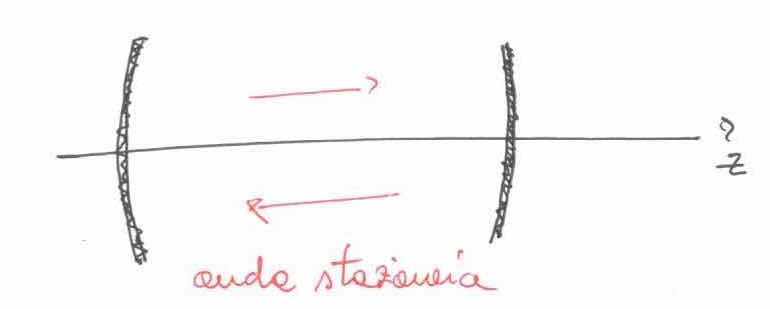
\includegraphics[height=4cm]{images/8}
\end{figure}
\item Risonatori ad anello
\begin{figure}[H]
\centering
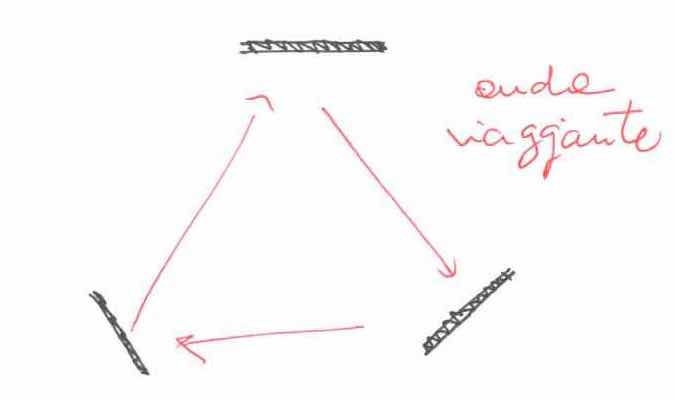
\includegraphics[height=4cm]{images/9}
\end{figure}
\end{itemize}
I risonatori ottici hanno perdite, l'energia può fuoriuscire dal risonatore. Le principali cause di perdite sono:
\begin{description}
\item [Perdite diffrattive] - dovute al fatto che la cavità è aperta.
\item [Perdite di accoppiamento] - dovute alla riflettività $R < 100\%$ dello spettro di uscita.
\item [Perdite di assorbimento/scattering] - dovute agli elementi ottici in cavità.
\end{description}
Le perdite fanno si che le soluzioni d'onda che soddisfano le condizioni al contorno siano della forma:
\begin{equation*}
\*E(x,y,z,t) = \*U_{n,m,l}(x,y,z) \cos(\omega_{n,m,l} t) e^{\frac{t}{2\tau_c}} \quad t \geq 0
\end{equation*}
dove $\omega_{n,m,l}$ è la frequenza di risonanza del quasi-modo, $\*U_{n,m,l}(x,y,z)$ è il profilo di modo, e $\tau_c$ il tempo di vita dei fotoni in cavità del modo ($\tau_c$ in generale dipende dagli indici $n$,$m$,$l$).
Per $\tau_c$ finito, lo spettro di Fourier del campo $\*E$ è una lorentziana centrata in $\omega_{n,m,l}$ con larghezza proporzionale a $\frac{1}{\tau_c}$.
\begin{figure}[H]
\centering
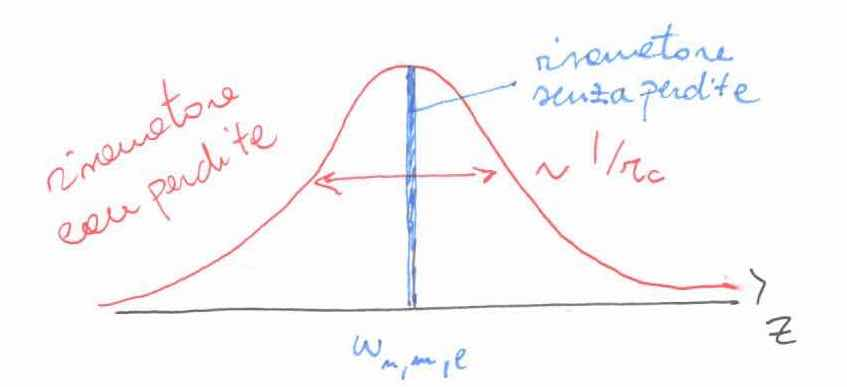
\includegraphics[height=4cm]{images/10}
\end{figure}
\noindent
\begin{example}
Calcolare la frequenza di risonanza di una cavità ottica costituita da due specchi metallici perfettamente riflettenti posti a distanza $L$. Si discutano inoltre le proprietà metalliche dei modi e.m. (onde stazionarie).
\begin{figure}[H]
\centering
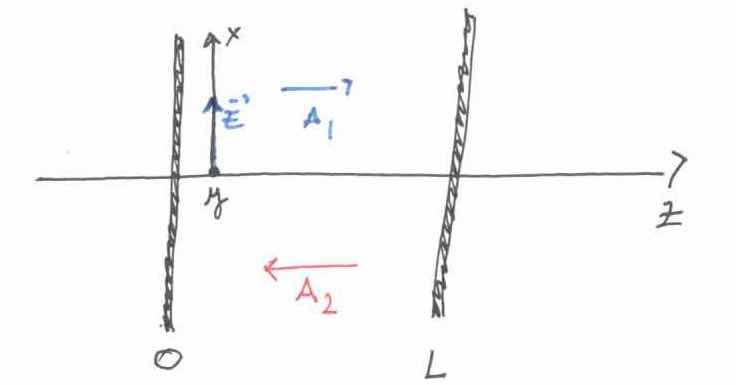
\includegraphics[height=4cm]{images/11}
\end{figure}
\noindent
Cerchiamo una soluzione della forma:
\begin{equation*}
\*E(x,y,z,t) = \frac{1}{2} \left[\underbrace{A_1 e^{i\omega t - ikz}}_\text{onda progressiva} + \underbrace{A_2 e^{i\omega t + ikz}}_\text{onda regressiva} + \,c.c.\right] \widehat{u}_x
\end{equation*}
con $k \equiv \frac{\omega}{c}$.
Le condizioni al contorno, sui due specchi sono:
\begin{equation*}
E_x(z=0,t) \equiv 0 \qquad E_y(z=0,t) \equiv 0
\end{equation*}
che implicano:
\begin{equation*}
\begin{cases}
A_1 e^{i\omega t} + A_2 e^{i\omega t} + c.c. \equiv 0 \qquad \forall t\\
A_1 e^{i\omega t} e^{-ikL} + A_2 e^{i\omega t} e^{ikL} + c.c. \equiv 0 \qquad \forall t
\end{cases}
\end{equation*}
e cioè, necessariamente:
\begin{equation*}
\begin{cases}
A_1 + A_2 = 0\\
A_1 e^{-ikL} + A_2 e^{ikL} = 0
\end{cases}
\end{equation*}
Tale sistema ha soluzione nulla se:
\begin{equation*}
\begin{bmatrix}
1	&	1\\
e^{-ikL}	&	e^{ikL}
\end{bmatrix} = 0
\end{equation*}
cioè $\sin(kL) = 0$ per $kL = n\pi$.
\begin{empheq}[box=\eqbox]{equation*}
\omega_n = kc = \frac{n\pi}{L} c \qquad\text{Frequenza di risonanza con n indice longitudinale}
\end{empheq}
Se $\w=\omega_n$, il campo elettrico vale:
\begin{align*}
\*E(x,y,z,t) &= \frac{1}{2} \left[A_1 e^{i\omega_n t - ik_n z} + A_2 e^{i\omega_n t + ik_n z} + c.c.\right]\\
&= \frac{1}{2} \left[A_1 e^{i\omega_n t} \left(e^{-ik_n z} - e^{ik_n z}\right) + c.c.\right]\\
&= -iA_1 e^i\omega_n t \sin(k_n z) + c.c.
\end{align*}
Posto $E_0 \equiv -2iA_1$ che assumo reale, si ha:
\begin{empheq}[box=\eqbox]{equation*}
E_x(z,t) = E_0 \sin(k_n z) \cos(\omega_n t) \qquad \text{onda stazionaria}
\end{empheq}
%disegno
ci sono $(n+1)$ nodi e $n$ vertici. La condizione di quantizzazione di $k$ si interpreta facilmente pensando alla corda vibrante.
\begin{equation*}
L = n \frac{\l}{2} \quad \text{con} \quad n=1,2,3...
\end{equation*}
Essendo $k = \frac{2\pi}{\l}$ questa condizione equivale a:
\begin{equation*}
L = n\frac{2\pi}{k} \frac{1}{2} = \frac{n\pi}{k} \quad \rightarrow \quad k = \frac{n\pi}{L}
\end{equation*}
\end{example}
\begin{example}
Calcolare i modi e le frequenze di risonanza di una risonatore ad anello a specchi piani in approssimazione di onda piana. Si indichi con $L$ il perimetro dell'anello.
\begin{figure}[H]
\centering
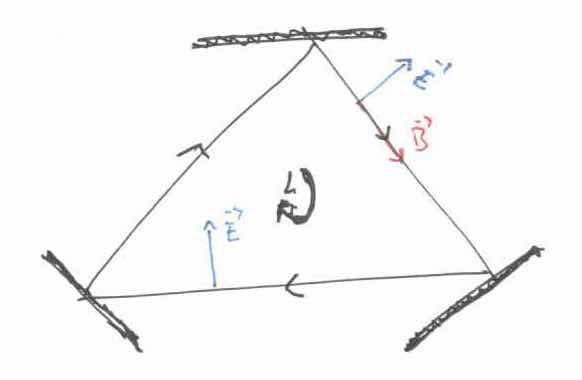
\includegraphics[height=4cm]{images/13}
\end{figure}
\noindent
Detto $z$ l'asse sghembo che descrive il perimetro dell'anello, cerco una soluzione dell'onda viaggiante lungo $z$:
\begin{equation*}
\*E(x,y,z,t) = \frac{1}{2} \left[Ae^{i\omega t -ikz} + c.c. \right] \widehat{u}_x
\end{equation*}
Essendo $z=0$ e $z=L$ i medesimi piani, $E$ in $z=0$ e $z=L$ deve assumere lo stesso valore per ogni $t$, e cioè deve essere soddisfatte le condizioni di autoconsistenza:
\begin{equation*}
E_x(z=0,t) \equiv E_x(z=L, t)
\end{equation*}
e cioè:
\begin{equation*}
A e^{i\omega t} + c.c. \equiv A e^{i\omega t - ikL} + c.c. \quad \forall t
\end{equation*}
che implica necessariamente:
\begin{equation*}
e^{-ikL} = 1
\end{equation*}
cioè:
\begin{equation*}
kL = 2n\pi \qquad \begin{cases}
k = k_n = \frac{2n\pi}{L}\\
\omega = \omega_n = \frac{2\pi c}{L} n
\end{cases}
\end{equation*}
$\nu_n = \frac{cn}{L}$ frequenza di risonanza del risonatore ad anello.

\begin{os}
La frequenza di risonanza longitudinale di un
Fabry-Perot di lunghezza $L$ è $\D\omega = \frac{\pi c}{L}$.
\end{os}
\begin{figure}[H]
\centering
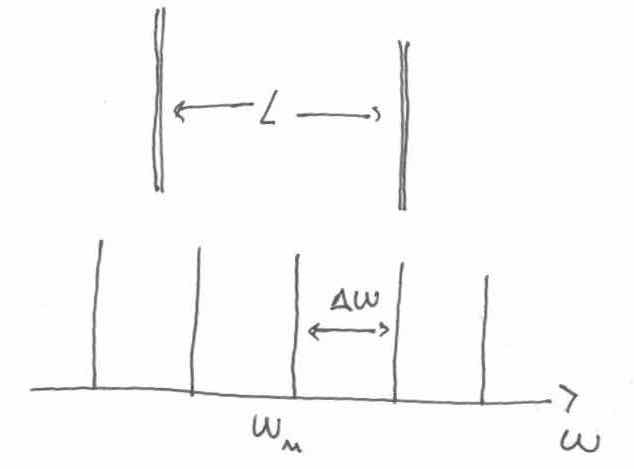
\includegraphics[height=4cm]{images/14}
\end{figure}
\noindent
Per una cavità ad anello $\D\omega = \frac{2\pi c}{L}$.
\begin{figure}[H]
\centering
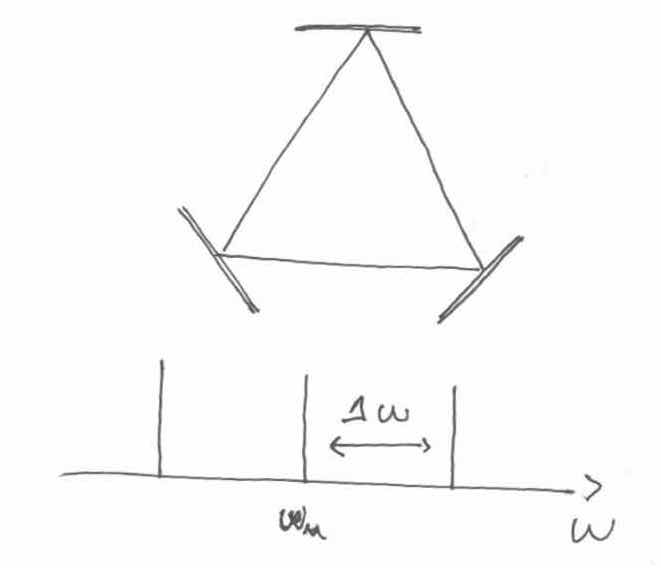
\includegraphics[height=4cm]{images/15}
\end{figure}
\end{example}

\begin{example}
Calcolare il numero di modi che cadono sotto la riga di guadagno di un mezzo attivo laser, con larghezza di riga $\D\nu_0$, nei seguenti casi:
\begin{enumerate}
\item cavità cilindrica chiusa di lunghezza $L$ e raggio $a$ con pareti metalliche perfettamente riflettenti
\item cavità aperta costituita dalla precedente rimuovendo la superficie laterale del cilindro.
\end{enumerate}
\begin{figure}[H]
\centering
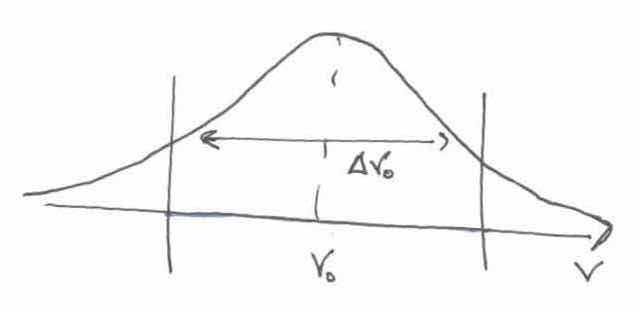
\includegraphics[height=4cm]{images/16.jpg}
\end{figure}
\begin{enumerate}
\item È noto che, per una cavità chiusa di volume $V$, la densità spettrale dei modi e.m. della cavità vale:
\begin{equation*}
\rho(\nu) = \frac{8\pi \nu^2 V}{c^3}
\end{equation*}
cioè $\rho(\nu) d\nu$ è il numero di modi con frequenza compresa tra $\nu$ e $\nu + d\nu$.
Quindi:
\begin{equation*}
N^{(closed)} = \rho(\nu_0) \D \nu_0 = \frac{8\pi \nu_0^2 V}{c^3} \D\nu_0
\end{equation*}
\item In questo caso i modi con basse perdite sono solo onde che si propagano lungo l'asse $z$. Le figure di tali modi sono equispaziati di:
\begin{equation*}
\D\nu = \frac{\D\omega}{2\pi} = \frac{c}{2L}
\end{equation*}
\begin{equation*}
N^{(open)} = \left\lfloor \frac{\D \nu_0}{\D \nu} \right\rfloor = \frac{\D \nu_0}{\frac{c}{2L}}
\end{equation*}
Calcolo il rapporto tra il numero di modi nei due casi:
\begin{equation*}
\frac{N^{(closed)}}{N^{(open)}} = \frac{\frac{8\pi \nu_0^2}{c^3} \D \nu_0 \pi a^2 L}{\frac{\D \nu_0}{\frac{c}{2L}}} = ... = \left( \frac{2\pi a}{\l_0} \right)^2
\end{equation*}
\end{enumerate}

\begin{exercise}
Si consideri un laser $HeNe$ con i seguenti parametri costruttivi:\\
$L = 50 cm$ $\l_0 = 633 nm$ $2a = 3 mm$ $\D\nu_0 = 1.7GHz$\\
Utilizzando quanto visto in precedenza si ha:
\begin{equation*}
N^{(open)} \simeq 6
\end{equation*}
\begin{equation*}
\frac{N^{(closed)}}{N^{(open)}} = 1.2 \cdot 10^9
\end{equation*}
Con una cavità chiusa ci sarebbero una quantità enorme di modi che verrebbero amplificati risultando in una sorgente non monocromatica. Viceversa, nel caso di cavità aperta i modi sono solamente 6. Ecco spiegato perché i laser sono costituiti da cavità aperte e non chiuse.
\end{exercise}
\end{example}

\section{Teoria geometrica dei risonatori ottici: Teorema di stabilità}
Considero un risonatore a cavità lineare costituita da due specchi sferici terminali, di raggi di curvatura $R_1$ e $R_2$, posti a distanza $L$. Tra i due specchi, in generale, possono esservi altri elementi ottici (lenti). L'asse ottico $z$ del risonatore è la retta che congiunge i centri degli specchi.
%disegno
Preso un piano $\gamma$ perpendicolare a $z$ interno al risonatore, studiamo la propagazione di un raggio parassiale che rimbalza avanti e indietro tra i due specchi.
Sia $(r_0,r_0'), (r_1,r_1'), \dots, (r_n,r_n'), \dots$ i parametri parassiali del raggio, quando attraverso il piano $\gamma$ da sinistra a destra, all'n-esimo round-trip.

Definizione
Il risonatore si dice stabile secondo l'ottica geometrica se, fissati $(r_0,r_0')$ ad arbitrio, $r_n$ e $r_n'$ non divergono se $n\rightarrow\infty$. Cioè, il risonatore è stabile se è in grado di intrappolare i raggi che rimbalzano tra i due specchi.

Si noti che la propagazione di un raggio luminoso tra i due specchi del risonatore è equivalente alla propagazione di un raggio nella lensguide così costruita.
%disegno
La matrice trasmissione di uno specchio in riflessione è uguale a quella di una lente in trasmissione se $f = \frac{R}{2}$.\\
Specchio
\begin{equation*}
\begin{bmatrix}
1	&	0\\
-\frac{2}{R}	&	1
\end{bmatrix}
\end{equation*}
Lente
\begin{equation*}
\begin{bmatrix}
1	&	0\\
-\frac{1}{f}	&	1
\end{bmatrix}
\end{equation*}
Vale il fondamentale teorema di stabilità: sia la matrice ABCD la matrice round-trip del risonatore rispetto al piano $\gamma$, cioè la matrice a raggi del piano $z=0$ al piano $z=2L$ nella lensguide equivalente. Allora il risonatore è stabile secondo l'ottica geometrica se è soddisfatta la seguente
\begin{equation*}
\left| \frac{A+D}{2} \right| < 1
\end{equation*}
Infatti, per definizione di matrice ABCD, si ha:
\begin{equation*}
\begin{bmatrix}
r_1\\
r_1'
\end{bmatrix} = 
\begin{bmatrix}
A	&	B\\
C	&	D
\end{bmatrix}
\begin{bmatrix}
r_0\\
r_0'
\end{bmatrix},
\begin{bmatrix}
r_2\\
r_2'
\end{bmatrix} = 
\begin{bmatrix}
A	&	B\\
C	&	D
\end{bmatrix}
\begin{bmatrix}
r_1\\
r_1'
\end{bmatrix} =
\begin{bmatrix}
A	&	B\\
C	&	D
\end{bmatrix}^2
\begin{bmatrix}
r_0\\
r_0'
\end{bmatrix},\dots
\begin{bmatrix}
r_n\\
r_n'
\end{bmatrix}
=\begin{bmatrix}
r_1\\
r_1'
\end{bmatrix} = 
\begin{bmatrix}
A	&	B\\
C	&	D
\end{bmatrix}^n
\begin{bmatrix}
r_0\\
r_0'
\end{bmatrix}
\end{equation*}
Dalla definizione di stabilità, il risonatore è stabile se:
\begin{equation*}
|r_n| < \infty, \qquad |r_n'| < \infty
\end{equation*}
per $n\rightarrow \infty$, qualunque sia $(r_0, r_0')$.
Posto $M \equiv \begin{bmatrix}
A	&	B\\
C	&	D
\end{bmatrix}$, detta $\begin{bmatrix}
\l_1	&	0\\
0	&	\l_2
\end{bmatrix}$ e $T$ la matrice diagonale $\Lambda$ degli autovalori $(\l_1,\l_2)$ di $M$ e dei corrispondenti autovettori
\begin{equation*}
MT = T\Lambda
\end{equation*}
se $T$ è invertibile, ho:
\begin{equation*}
M = T\Lambda T^{-1}
\end{equation*}



e poiché
\begin{equation*}
\Lambda^n = \begin{bmatrix}
\l_1	&	0\\
0	&	\l_2
\end{bmatrix}^n = \begin{bmatrix}
\l_1^n	&	0\\
0	&	\l_2^n
\end{bmatrix}
\end{equation*}
si ha
\begin{equation*}
\begin{bmatrix}
r_n\\
r_n'
\end{bmatrix} =
T\begin{bmatrix}
\l_1^n	&	0\\
0	&	\l_2^n
\end{bmatrix}
T^{-1}\begin{bmatrix}
r_0\\
r_0'
\end{bmatrix}
\end{equation*}
Per $n\rightarrow\infty$, $|r_n|$ e $r_n'$ sono limitati se e solo se:
\begin{equation*}
|\l_1| \leq 1, \qquad 
\end{equation*}
Calcolo $\l_1$ e $\l_2$
\begin{equation*}
\begin{bmatrix}
\l_1	&	0\\
0	&	\l_2
\end{bmatrix} = 0
\end{equation*}
\begin{align*}
&(\l-A)(\l-D)-BC = 0\\
&\l^2-(A+D)\l+\underbrace{AD-BC}_\text{det M = 1} = 0
\end{align*}
Introdotto l'angolo $\theta$ così definito:
\begin{equation*}
\cos \theta \equiv \frac{A+D}{2}
\end{equation*}
\begin{equation*}
\l^2 - 2\cos\theta\l + 1 = 0, \quad \l_{1,2} = \cos\theta \pm \sqrt{\cos^2\theta -1} = \cos\theta \pm i\sin\theta = e^{\pm i\theta}
\end{equation*}
cioè:
\begin{equation*}
\l_{1,2} = e^{\pm i\theta}
\end{equation*}
Distinguo tre casi:
\begin{enumerate}
\item $\left|\frac{A+D}{2}\right|<1$, $\theta$ reale, $|\l_1|=|\l_2|=1$ e il risonatore è stabile.
\item $\frac{A+D}{2}>1$, $\theta = i\psi$ con $cosh \psi=\frac{A+D}{2}$, $psi$ reale. Per cui $|\l_1|= e^{i\theta}=e^{-\psi}$, $\l_2=e^\psi$ uno dei due autovalori ha modulo maggiore di uno quindi il risonatore è instabile.
\item $\frac{A+D}{2}<-1$, posto $\theta=i\psi+\pi$ ho $cosh \psi=-\frac{A+D}{2} = \left|\frac{A+D}{2}\right|$ cioè $psi$ reale. In tal caso: $\l_{1,2}= e^{\pm i\theta}=e^{\pm i\theta \mp \psi} = -e^{\mp\psi}$. Ancora, uno dei due autovalori ha modulo maggiore di uno quindi il risonatore è instabile.
\end{enumerate}

Esempio notevole: risonatore a die specchi sferici
%disegno
Considero due specchi sferici di raggio di curvatura $R_1$ e $R_2$ a distanza $L$ fra i quali c'è il vuoto. Scelto $\gamma$ come in figura, la lensguide equivalente è:
%disegno
La matrice $M$ di round trip rispetto a $\gamma$ vale:
\begin{equation*}
M = \begin{bmatrix}
1	&	0\\
-\frac{2}{R_1}	&	1
\end{bmatrix}
\begin{bmatrix}
1	&	L\\
0	&	1
\end{bmatrix}
\begin{bmatrix}
1	&	0\\
-\frac{2}{R_2}	&	1
\end{bmatrix}
\begin{bmatrix}
1	&	L\\
0	&	1
\end{bmatrix} = \dots
\end{equation*}
da cui:
\begin{equation*}
\frac{A+D}{2} = 2(1-\frac{L}{R-1})(1-\frac{L}{R_2}) - 1
\end{equation*}
Introdotti i parametri $g_1, g_2$ del risonatore così definiti:
\begin{equation*}
g_1 \equiv 1-\frac{L}{R_1}, \quad g_2 \equiv 1-\frac{L}{R_2}
\end{equation*}
la condizione di stabilità diventa
\begin{equation*}
-1 < 2g_1 g_2 -1 <1
\end{equation*}
cioè:
\begin{equation*}
0 < g_1g_2 < 1 \qquad \text{Condizione di stabilità (per questo caso)}
\end{equation*}
Diagramma di stabilità del piano $(g_1,g_2)$
%disegno
Caso notevole:
risonatori simmetrici ha $R_1=R_2=R$, da cui $g_1=g_2=1-\frac{L}{R}$
Si noti che esistono 3 risonatori simmetrici al limite della stabilità:
\begin{enumerate}
\item $g_1=g_2=1$ cioè $R=0$: Risonatore piano-piano
%disegno
Non è stabile
\item $g_1=g_2=0$ cioè $R=L$: Risonatore confocale
%disegno
è stabile e ogni raggio ritorna su se stesso dopo due round trip
\item $g_1=g_2 = -1$ cioè $L=2R$: Risonatore concentrico
%disegno
È instabile
\end{enumerate}
Osservazione
La teoria svolta, fino al teorema di stabilità incluso, (escludere esempio notevole) vale




\section{Teoria ondulatoria dei risonatori:  modi e frequenze di risonanza}
Considero un risonatore a cavità lineare, costituito da due specchi terminali di raggi di curvatura $R_1$ e $R_2$ posti a distanza $L$, fra gli specchi possono essere interposti altri elementi (lenti). Supponiamo che:
\begin{enumerate}
\item Gli specchi sono infinitamente estesi (trascuro gli effetti di bordo e perdite diffrattive)
\item  Suppongo gli specchi riflettenti al 100\% (i quasi-modi sono modi)
\item Considero onde e.m. parassiali in approssimazione scalare (modi quasi TEM). La propagazione di un campo e.m. intrappolato fra i due specchi, rappresentabile dalla sovrapposizione o interferenza di due onde parassiali contropropagantesi può essere descritta in maniere sostanzialmente equivalente alla propagazione di un'onda viaggiante nella lens guide equivalente.
%disegno
Tracciamo la lens guide (unfolding):
%disegno
\end{enumerate}
Detto $\*E(x,y,z,t) = \frac{1}{2} [u(x,y,z) e^{i\omega t-ikz} + c.c.] \*u_x$ il campo che si propaga nella lensguide ho un inviluppo $u(x,y,z)$ che in funzione di $z$ varia in accordo dell'integrale generalizzato di KHF. Nel problema originale, i percorsi $z=0$ e $z=2L$ sono il medesimo piano $\gamma$; pertanto, per monodromia, deve aversi:
\begin{equation*}
E_x(x,y,0,t) \equiv E_x(x,y,2L,t) \qquad \forall t
\end{equation*}
condizione di autoconsistenza

ovvero:
\begin{equation*}
u(x,y,0) = u(x,y,2L) e^{-2ikL}
\end{equation*}
Del resto, detta ABCD la matrice di roundtrip del risonatore rispetto al piano $\gamma$, si ha:
\begin{equation}
u(x,y,2L) = \iintinf u(x_1,y_1,0)K(x,x_1y,y_1)dx_1dy_1
\end{equation}
dove $K \equiv \frac{i}{\l B} e^{-\frac{ik}{2B} [A(x_1^2 + y_1^2) + D(x^2 + y^2) - 2xx_1 - 2yy_1]}$ è il nucleo (kernel) dell'integrale generalizzato di KHF. Sinteticamente scrivo:
\begin{equation*}
u(x,y,2L) = \widehat{K} u(x,y,0)
\end{equation*}
dove $\widehat{K}$ è l'operatore integrale di KHF.
La condizione di autoconsistenza è quindi:
\begin{equation*}
u(x,y,0) = e^{-2ikL} \widehat{K} u(x,y,0)
\end{equation*}
cioè:
\begin{empheq}[box=\eqbox]{equation*}\label{eq: }
\widehat{K}u(x,y,0) = \sigma u(x,y,0)
\end{empheq}
con $\sigma \equiv e^{2ikL}$.
Ciò significa che le eventuali soluzioni monocromatiche parassiali a frequenza $\w$ che soddisfano il problema e.m. tra i due specchi e le condizioni al contorno imposte dagli specchi sono le autofunzioni dell'operatore $\widetilde{K}$ con autovalori $\sigma = e^{2ikL}$ (eq.di Fredholm). Cerchiamo una soluzione dell'equazione agli autovalori della forma:
\begin{equation*}
u(x,y,0) = u_0 H_l\left(\frac{\sqrt{2}x}{w_1}\right)H_m\left(\frac{\sqrt{2}y}{w_1}\right) e^{-i\frac{k(x^2 + y^2)}{2q_1}}
\end{equation*}
cioè con distribuzione di Gauss-Hermite, dove $\Im{\frac{1}{q_1}}<0$. Sappiamo che:
\begin{equation*}
\widehat{K}u(x,y,0) = \frac{u_0}{\left(A+\frac{B}{q_1}\right)^{1+l+m}} H_l\left(\frac{\sqrt{2}x}{w}\right)H_m\left(\frac{\sqrt{2}y}{w}\right) e^{-i\frac{k(x^2 + y^2)}{2q}}
\end{equation*}
dove $q$ è dato dalla legge ABCD $q = \frac{Aq_1 + B}{Cq_1 + D}$
Imponiamo la \eqref{} \begin{equation*}
\widehat{K}u(x,y,0) = \sigma u(x,y,0)
\end{equation*}
Ciò implica:
\begin{equation*}
\begin{cases}
q=q_1\\
\sigma = \frac{1}{\left(A + \frac{B}{q_1}\right)^{1+l+m}}
\end{cases}
\end{equation*}
Studiamo le equazioni:
\begin{enumerate}
\item $q=q_1$ e cioè $q_1 = \frac{Aq_1 + B}{Cq_1 + D}$ ovvero:
\begin{equation*}
Aq + B = Cq^2 + Dq
\end{equation*}
o anche
\begin{equation*}
\frac{A}{q} + \frac{B}{q^2} = c +\frac{D}{q}, \quad B\left(\frac{1}{q}\right)^2 + (A-D)\left(\frac{1}{q}\right) -C = 0
\end{equation*}
Le soluzioni sono:
\begin{equation*}
\left(\frac{1}{q}\right)_{\pm} = -\frac{A-D}{2B} \pm \frac{1}{B}\sqrt{\left(\frac{A-D}{2}\right)^2 + BC}
\end{equation*}
Osservando che:
\begin{align*}
\left(\frac{A-D}{2}\right)^2 + BC &= \frac{A^2 +D^2 -2AD + 4BC}{4}\\
&= \frac{A^2 + D^2 - 2AD + 4(AD-1)}{4}\\
&= \frac{(A+D)^2 -4}{4}\\
&= \cos^2\theta -1 
\end{align*}
ricordando l'Ansatz $\cos\theta \equiv \frac{A+D}{2}$.
Pertanto:
\begin{equation*}
\left(\frac{1}{q}\right)_{\pm} = - \frac{A-D}{2B} \pm \frac{i\sin\theta}{B}
\end{equation*}
Le soluzioni accettabili sono quelle $Im{\frac{1}{q}}<0$ per confinamento. Osserviamo che, se $\left|\frac{A+D}{2}\right|>1$, $\theta = i\psi$ oppure $\theta=i\psi +\pi$ con $\psi$ reale e quindi $i\sin\theta$ reale. Per cui quando $Im{\frac{1}{q}}_\pm = 0$. Non ci sono soluzioni accettabili.
Se il risonatore è instabile secondo l'ottica geometrica (vedi. Th di stabilità) l'eq. agli autovalori di Fredholm non ha soluzioni in $L^2$: non ci sono modi e.m. confinati.
Se invece $\left|\frac{A+D}{2}\right|<1$, $\sin\theta$ è reale, $\Im{\frac{1}{q}_\pm}= \pm\frac{\sin\theta}{B}$ e quindi esiste una e una sola soluzione accettabile.
\item Seconda equazione:
\begin{align*}
e^{2ikL} &= \frac{1}{\left(A + \frac{B}{q_1}\right)^{1+l+m}}\\
&= \frac{1}{\left(A + \frac{A-D}{2}\pm i\sin\theta\right)^{1+l+m}}\\
&= \frac{1}{\left(\cos \theta \pm \sin \theta\right)^{1+l+m}}\\
&= \frac{1}{e^{\pm i\theta(i+l+m)}}
\end{align*}
cioè:
$e^{2ikL} = e^{\mp i\theta(1+l+m)}$ che implica $2kL = \mp \theta(1+l+m) + 2\pi n$ con $n$ intero. $k = \frac{\pi n}{L} \mp \frac{\theta}{2L}(1+l+m)$. $\nu = \frac{\omega}{2\pi} = \frac{kc}{2\pi} = \frac{c}{2L} \left[n \mp \frac{\theta}{2\pi}(1+l+m)\right]$
cioè:
\begin{equation*}
\nu_{n,l,m} = \frac{c}{2L} \left[n \mp \frac{\theta}{2\pi}(1+l+m)\right]
\end{equation*}
frequenza di risonanza

$\nu$ dipende da tre indici:
\begin{description}
\item [n] indice longitudinale
\item [l,m] indici trasversali
\end{description}

\end{enumerate}

Esempio: frequenza di risonanza del risonatore confocale

\begin{equation*}
\nu_{n,l,m} = \frac{c}{2L} \left[n \mp \frac{\theta}{2\pi}(1+l+m)\right]
\end{equation*}
con $\cos\theta = \frac{A+D}{2}$.
Calcolo matrice ABCD per confocale.
%disegno
%disegno
\begin{equation*}
M = \begin{bmatrix}
A	&	B\\
C	&	D
\end{bmatrix}
=\begin{bmatrix}
1	&	0\\
-\frac{2}{R}	&	1
\end{bmatrix}\begin{bmatrix}
1	&	R\\
0	&	1
\end{bmatrix}\begin{bmatrix}
1	&	0\\
-\frac{2}{R}	&	1
\end{bmatrix}\begin{bmatrix}
1	&	R\\
0	&	1
\end{bmatrix}=\begin{bmatrix}
-1	&	0\\
0	&	-1
\end{bmatrix}=-I
\end{equation*}
Si noti che $M^2 = I$: ciò significa che, in un confocale, dopo due round-trip ogni distribuzione di campo e.m. ritorna ad essere uguale a se stessa.
Per il confocale, o vicino alla confocalità, il valore di $\theta$ vale:
\begin{equation*}
\cos\theta = \frac{A+D}{2}\simeq -1
\end{equation*}
cioè $\theta=\pi$. Quindi:
\begin{equation*}
\nu_{n,l,m} = \frac{c}{2L} \left[n + \frac{1}{2}(1+l+m)\right] = \frac{c}{4L} \left[2n + (1+l+m)\right]
\end{equation*}
%disegno
Si noti che al variare di $n,l,m$, $\nu_{n,l,m}$ descrive un pettine di frequenze con i centri equispaziati di $\frac{c}{4L}$ (v. figura). Ogni frequenza di risonanza è infinite volte degenere.
Osservazione: si noti che se applico la condizione di autoconsistenza nel confocale e cioè la prima eq di ieri: $q = \frac{Aq_1 + B}{Cq_1 + D}$
essendo $A=D=-1$, $B=C=0$ si ha: $q=q$ identità.

Esercizio 1
i) Detta ABCD la matrice di round trip rispetto a $\gamma$ il parametro $q$ del modo $TEM_{00}$ del risonatore in $\gamma$ soddisfa la condizione di autoconsistenza $q = \frac{Aq_1 + B}{Cq_1 + D}$ ovvero $\left(B\frac{1}{q}\right)^2 + (A-D)\frac{1}{q} - C = 0$. Su $\gamma$, il raggio di curvatura $R_\gamma$ e lo spot size $w_\gamma$ del modo $TEM_{00}$ sono dati dall'Ansatz:
\begin{equation*}
\frac{1}{q} = \frac{1}{R_\gamma} -i\frac{\l}{\pi w_\gamma^2}
\end{equation*}
Su $\gamma$ il modo ha un beam waist se $R_\gamma=\infty$, cioè $q$ puramente immaginario. Essendo:
\begin{equation*}
\frac{1}{q}_\pm = -\frac{A-D}{2B} \pm i\frac{\sin\theta}{B}
\end{equation*}
per risonatore stabile $\theta$ reale, quindi $\Re{\frac{1}{q}}=0$ se e solo se $A=D$.\\
ii) Dimostrare che la semi traccia della matrice ABCD non dipende dal piano $\gamma$.\\
%disegno
Siano $\gamma$ e $\beta$ due piani interni al risonatore. Facciamo la lensguide rispetto a $\gamma$:
%disegno
Dette $M_\gamma$ e $M_\beta$ le matrici di round trip rispetto ai piani $\gamma$ e $\beta$ si ha evidentemente:
\begin{equation*}
M_\gamma = M_2M_1 \qquad M_\beta = M_1M_2
\end{equation*}
Essendo il prodotto di matrici non commutativo in generale $M_\beta \neq M_\gamma$.\\
Per la proprietà di invarianza della traccia del prodotto di matrici per permutazioni cicliche, ad es.
\begin{equation*}
Tr(ABC) = Tr(CAB) = Tr(BCA)
\end{equation*}
si ha $Tr(M_\gamma) = Tr(M_\beta)$.\\
\\
Esercizio 2
Laser Ti:sapphire ($\l=780nm$)
perimetro $L$
$f = 2cm$\\
i) Calcolare $L=L_{max}$ per cui $L<L_{max}$ il risonatore è stabile.
Scelto il piano $\gamma$ come in figura, la matrice ABCD di transito nell'anello da $\gamma\rightarrow\gamma$ vale:
\begin{equation*}
\begin{bmatrix}
A	&	B\\
C	&	D
\end{bmatrix}
=\begin{bmatrix}
1	&	\frac{L}{2}\\
0	&	1
\end{bmatrix}\begin{bmatrix}
1	&	0\\
-\frac{1}{f}	&	1
\end{bmatrix}\begin{bmatrix}
1	&	\frac{L}{2}\\
0	&	1
\end{bmatrix}=\begin{bmatrix}
1-\frac{L}2f{}	&	L-\frac{L^2}{4f}\\
-\frac{1}{f}	&	1-\frac{L}{2f}
\end{bmatrix}
\end{equation*}
Per il th di stabilità, il risonatore è stabile:
\begin{equation*}
-1 < \frac{A+D}{2} < 1
\end{equation*}
cioè:
\begin{equation*}
-1 < 1-\frac{L}{2f} < 1, \quad \begin{cases}
1 - \frac{L}{2f} < 1 \rightarrow \frac{L}{2f} > 0 \text{ovvia}\\
1-\frac{L}{2f} > -1 \rightarrow \frac{L}{2f} < 2 \rightarrow L_{max} =4f
\end{cases}
\end{equation*}
ii) Calcolare la posizione del punto di vita del fascio dentro l'anello, la dimensione di macchia e la dimensione di macchia della lente nel caso in cui $L_{max} = \frac{L}{2} = 2f$.
Il parametro $q$ del modo $TEM_00$ al piano $\gamma$ si ottiene dalla condizione di autoconsistenza: $q = \frac{Aq_1 + B}{Cq_1 + D}$
\begin{equation*}
Cq^2 + Dq = Aq + B, \quad q^2=\frac{B}{C} = \frac{L - \frac{L^2}{4f}}{-\frac{1}{f}} = \frac{2f - f}{-\frac{1}{f}}
\end{equation*}
cioè $q^2 = -f^2$, ovvero $q = if$.
Essendo $q$ puramente immaginario su $\gamma$, $R_\gamma=\infty$ cioè su $\gamma$ il fronte di fase è piano e il modo $TEM_{00}$ ha il suo beam waist. Quanto vale $w_0$ nel punto di vita? Ricordo che, per fascio gaussiano in propagazione libera con beam waist in $z=0$, $q(z) = z +iz_R$ dove $z_R \equiv \frac{\pi w_0^2}{\l}$. Pertanto:
\begin{equation*}
\frac{\pi w_0^2}{\l} = f, w_0 = \sqrt{\frac{\l f}{\pi}} = 705 \mu m
\end{equation*}
Per calcolare $w_\beta$ osservo che dal beam waist sul piano $\gamma$ il fascio $TEM_{00}$ si propaga in propagazione libera fino a $\beta$. Pertanto:
\begin{equation*}
w_\beta = w_\gamma \sqrt{1+ \left(\frac{\frac{L}{2}}{f}\right)^2} = \sqrt{2}w_\gamma
\end{equation*}
cioè:
\begin{equation*}
w_\beta = \sqrt{2}w_\gamma = \sqrt{\frac{2\l f}{\pi}} \simeq 997 \mu m
\end{equation*}







\section{Risonatori con perdite: $\tau_c$ e fattore di qualità Q di un risonatore}
Considero cavità ottica lineare con specchi di riflettività $R_1$ e $R_2$. Preso u piano $\gamma$ interno al risonatore e detta $I(T)$ l'intensità al tempo $t$ dell'onda progressiva al piano $\gamma$ e al tempo $t$, si ha:
\begin{equation*}
I(t+T_R) = R_1R_2 (1-T_1)^2 I(t)
\end{equation*}
dove $T_R \equiv \frac{2L_c}{c_0}$ è il tempo di round-trip della luce nel risonatore, $L_c$ lunghezza ottica $L_c = \int_0^L n(z) dz$ $T_1$ trasmissione fittizia che tiene conto delle perdite interne per singolo transitorio.
Cerco una soluzione dell'equazione alle differenze con l'Ansatz:
\begin{equation*}
I(t) = I(0) e^{-\frac{t}{\tau_c}}
\end{equation*}
con $\tau_c$ costante di tempo (tempo di vita dei fotoni in cavità) da determinarsi. Sostituisco l'Ansatz:
\begin{equation*}
I(0) e^{-\frac{t+T_R}{\tau_c}} = R_1 R_2 (1 + T_1)^2 I(0)e^{-\frac{t}{\tau_c}}
\end{equation*}
e cioè
\begin{equation*}
e^{-\frac{T_R}{\tau_c}} = R_1 R_2 (1 + T_1)^2
\end{equation*}
da cui
\begin{equation*}
\frac{T_R}{\tau_c} = -\ln R_1 - \ln R_2 - 2 \ln(i-T_i)
\end{equation*}
Introdotte le cosiddette perdite logaritmiche (per singolo passaggio) del risonatore:
\begin{equation*}
\gamma \equiv \frac{\gamma_1 + \gamma_2}{2} + \gamma_i
\end{equation*}
con \begin{align*}
&\gamma_1 \equiv -\ln R_1\\
&\gamma_2 \equiv -\ln R_2\\
&\gamma_i \equiv -\ln (1-T_r)
\end{align*}
si ha $\frac{T_R}{\tau_c} = 2 \gamma$ ovvero $\tau_c = \frac{T_R}{2\gamma} = \frac{L_c}{c_0 \gamma}$ tempo di vita dei fotoni in cavità.
\\
Il campo elettrico in un punto del risonatore, decade, a causa delle perdite, con la relazione
\begin{equation*}
E(t) = E_0 \cos(\omega_c t) e^{-\frac{t}{2\tau_c}}
\end{equation*}
dove $\omega_c = \omega_{n,m,l}$ è una frequenza di risonanza calcolata nel caso di risonatori senza perdite. Lo spettro di potenza di $E(t)$ vale
\begin{equation*}
\tilde{E(\w)} \equiv \left| \int_0^\infty E_0 \cos(\omega_c t) e^{-\frac{t}{2\tau_c}} e^{i\omega t}
dt \right|^2 = \left( \frac{E_0}{2}\right)^2 \left| \int_0^\infty e^{i(\w+\omega_c-\frac{t}{2\tau_c}} + \int_0^\infty e^{i(\w-\omega_c-\frac{t}{2\tau_c}} dt \right|^2
\end{equation*}
Posto:
\begin{equation*}
F(\Omega) \equiv \int_0^\infty e^{i\Omega t - i\frac{t}{2\tau_c}} dt = \frac{1}{\frac{1}{2\tau_c - i\Omega}}
\end{equation*}
ho
\begin{equation*}
\tilde{E}(\w) = \left(\frac{E_0}{2}\right)^2 \left| F(\omega + \omega_c) + F(\omega - \omega_c)\right|^2 \approx \left(\frac{E_0}{2}\right)^2 \left|F(\omega + \omega_c)\right|^2 + \left|F(\omega - \omega_c)\right|^2
\end{equation*}cioè
\begin{equation*}
\tilde{E}(\w) = \frac{E_0^2}{4} \left[ \frac{1}{\left(\frac{1}{2\tau_c}\right)^2 + (\w+\omega_c)^2} + \frac{1}{\left(\frac{1}{2\tau_c}\right)^2 + (\w-\omega_c)^2}\right]
\end{equation*}
Si noti che, considerando le sole frequenze positive. $\tilde{E}(\w)$ è una loretziana con FWHM $ \D \omega_c = \frac{1}{\tau_c}$ ovvero $\D \nu_c = \frac{1}{2\pi\tau_c}$
%disegno
Per un risonatore con perdite, si definisce il fattore Q così:
\begin{equation*}
Q = 2\pi \cdot \frac{\text{energia del campo e.m. immagazzinata nel risonatore al tempo t}}{\text{energia persa in un ciclo ottico}}
\end{equation*}
Calcolo il num e il dem
Sia $\phi = \phi(t)$ il numero di elettroni di fotoni in cavità al tempo $t$. È evidente, come vederemo, che
\begin{equation*}
\phi8t) = \phi(0)e^{-\frac{t}{\tau_c}}
\end{equation*}
per cui
\begin{equation*}
num = \phi(t) \hbar \omega_c
\end{equation*}
e
\begin{equation*}
dem = \left| \frac{d\phi}{dt}\right| \hbar \omega_c \frac{2\pi}{\omega_0}
\end{equation*}
tenendo conto che $\left|\frac{d\phi}{dt}\right| = \frac{\phi}{\tau_C}$
si ha
\begin{equation*}
Q = 2\pi \cdot \frac{\phi(t) \hbar \omega_c}{\left|\frac{d\phi}{dt}\right| \hbar \omega_c \frac{2\pi}{\omega_0}} = 2\pi \cdot \frac{\phi(t)}{\frac{\phi(t)}{\tau_c} \frac{1}{\tau_c}} = 2\pi \tau_c \nu_c
\end{equation*}
cioè 
\begin{equation*}
Q = 2\pi \tau_c \nu_c = \frac{\nu_c}{\Delta \nu_c}
\end{equation*}
Esempio
Laser a HE-Ne ($\nu_c = \frac{c_0}{\l_c}$ con $\l = 633 nm$) $L_c \simeq = L = 90cm$ $R_1 = R_2 = 98\% = 0.98, T_i \approx 0$ Per cui
$\gamma_1 = -\ln R_1 = -\ln (1-T_1) \approx T_1 = 0.02$ $\gamma_2 = -\ln R_2 = \gamma_1 \approx 0.02$ $\gamma_i = -\ln (1-T_1) \approx 0$
\begin{equation}
\gamma = \frac{\gamma_1 + \gamma_2}{2} \simeq 0.02
\end{equation}
\begin{equation*}
\tau_c = \frac{L_c}{c_0\gamma} \simeq 150 ns
Q = \frac{\nu_c}{\D \nu_c} = \frac{2\pi \tau_c c_0}{\l_c} = 4.7 \cdot 10^8
\end{equation*}

Tema d'esame 8/2/2016
%disegno
Trascurare il diagramma di stabilità nel piano $(x_1, x_2)$ con $x_1 \equiv \frac{L_1}{f}$ e $x_2 \equiv \frac{L_2}{f}$
Il risonatore è in forma canonica, quindi esso è stabile se $A_1B_1C_1D_1 < 0$ essendo:
\begin{equation*}
\begin{bmatrix}
A_1	&	B_1\\
C_1	&	D_1
\end{bmatrix}
=\begin{bmatrix}
1	&	L_2\\
0	&	1
\end{bmatrix}\begin{bmatrix}
1	&	0\\
-\frac{1}{f}	&	1
\end{bmatrix}\begin{bmatrix}
1	&	L_1\\
0	&	1
\end{bmatrix}=\begin{bmatrix}
1-\frac{L_2}{f}	&	L_1+L_2-\frac{L_1L_2}{f}\\
-\frac{1}{f}	&	1-\frac{L_1}{2f}
\end{bmatrix}
\end{equation*}
è la one-way matrix da $\alpha \rightarrow \beta$. Perciò
\begin{equation*}
-\frac{1}{f} (1-\frac{L_2}{f})(1-\frac{L_1}{2f})(L_1+L_2-\frac{L_1L_2}{f}) < 0
\end{equation*}
ovvero
\begin{equation*}
(1-\frac{L_2}{f})(1-\frac{L_1}{2f})(L_1+L_2-\frac{L_1L_2}{f}) > 0
\end{equation*}
In funzione dei parametri $x_1$ ed $x_2$ ho:
\begin{equation*}
(1-x_2)(1-x_1)(x_1+x_2-x_1x_2) > 0
\end{equation*}
Limiti di stabilità
\begin{enumerate}
\item $x_1 = 1$
\item $x_2 = 1$
\item $x_1 + x_2 - x_1x_2 = 0$ cioè $x_2 = \frac{x_1}{x_1 - 1}$
\end{enumerate}
%disegno

Tema d'esame 6/7/2012
$\l = 1064 nm$ con cavità come in figura
%disegno
beam waist $\omega_0 0 200 \mu m$ $d = 3cm$

Calcolare R ed L.\\
Sfruttando la proprietà che in un risonatore a cavità lineare gli specchi terminali della cavità sono superfici equifase del modo $TEM_{00}$ ho:
\begin{equation*}
R(z) = z \left[1+\left(\frac{z_R}{z}\right)^2 \right]
\end{equation*}
con $z_c \equiv \frac{\pi \omega_0^2}{\l} = 11.81 cm$
e cioè
\begin{equation*}
R = d \left[1+\left(\frac{z_R}{z}\right)^2 \right] \simeq 49.5 cm
\end{equation*}
Posto $x \equiv L + d$ deve anche aversi:
\begin{equation*}
R = x \left[1+\left(\frac{z_R}{z}\right)^2 \right] 
\end{equation*}
e cioè
\begin{equation*}
R x = x^2 + z_R^2
\end{equation*}
$x^2 -R x + z_R^2 = 0$ che è un'equazione di secondo grado in x.
Le radici dell'equazione di secondo grado sono
\begin{equation*}
x_\pm = \frac{R}{2} \pm \sqrt{\left(\frac{R}{2}\right)^2 - x_R^2}
\end{equation*}
la soluzione $x_-$, la più piccola cl segno -, è evidentemente d.
La soluzione $x_+$, la più grande, + proprio $L + d$
Pertanto:
\begin{equation*}
L + d = \frac{R}{2} + \sqrt{\left(\frac{R}{2}\right)^2 - z_R^2}
\end{equation*}
ovvero
\begin{equation*}
L = \frac{R}{2} + \sqrt{\left(\frac{R}{2}\right)^2 - z_R^2} - d = \frac{R}{2} + \frac{R}{2} - d - d = R - 2d \simeq 43.5 cm
\end{equation*}